\documentclass[11pt, twoside]{book}
\usepackage[full]{leadsheets}
\usepackage[a4paper,  hmargin=1.5cm, vmargin=3cm]{geometry}
\usepackage{multicol}
\usepackage[polish]{babel}
\usepackage{array}
\usepackage{graphicx}
\usepackage{hyperref}
\usepackage{tocloft}
\usepackage{fancyhdr}
\usepackage{tikzpagenodes}
\usepackage{titlesec}
\thispagestyle{empty}

%\usepackage[default]{lato}
%\usepackage[T1]{fontenc}

\selectlanguage{polish}
\DeclareTranslation{Polish}{leadsheets/chorus}{Ref.}
\DeclareTranslation{Polish}{leadsheets/interlude}{Przej.}
\DeclareTranslation{Polish}{leadsheets/lyrics}{tekst}
\DeclareTranslation{Polish}{leadsheets/verse}{Zwr.}
%\DeclareTranslation{Polish}{leadsheets/capo}{Kapo}
\DeclareTranslation{Polish}{leadsheets/fret}{próg}

% Tytuł spisu treści
\addto\captionspolish{\renewcommand*\contentsname{Jakieś piosenki}}

\definesongtitletemplate{custom}{%
    \let\clearpage\relax
    \ifsongmeasuring%
        {\section*}
        {\section}%
        {\songproperty{title}}%
    \begingroup\footnotesize
        \begin{tabular}{%
                @{}
                >{\raggedright\arraybackslash}p{.5\linewidth}
                @{}
                >{\raggedleft\arraybackslash}p{.5\linewidth}
                @{}
            }
            \ifsongproperty{music}{%
                Muzyka: \songproperty{music} \\%
                }{}%
            \ifsongproperty{interpret}{%
                Interpretacja: \songproperty{interpret} \\%
                }{}%
            \ifsongproperty{capo}{%
                & \capo{} \\%
                }{}%
        \end{tabular}%
        \par
    \endgroup
}

\setleadsheets{%
    title-template = custom,
    verse/numbered,
    remember-chords=false,
    align-chords={l},
    capo-nr-format=arabic,
    bar-shortcuts
}

\renewcommand{\chaptermark}[1]{\markboth{#1}{}}

\fancypagestyle{plain}{%
    \fancyhf{}
    \fancyhead[L]{Jakieś piosenki}
    \fancyfoot[LE,RO]{\Large\thepage}
}
\fancypagestyle{szanty}{%
    \pagestyle{plain}
    %\fancyhf{}
    %\fancyhead[L]{Jakieś piosenki}
    \fancyhead[R]{Szanty}
    %\fancyfoot[LE,RO]{\Large\thepage}
    \fancyfoot[LO]{
\includegraphics[width=1.5cm]{images/kolo.png}}
    \fancyfoot[RE]{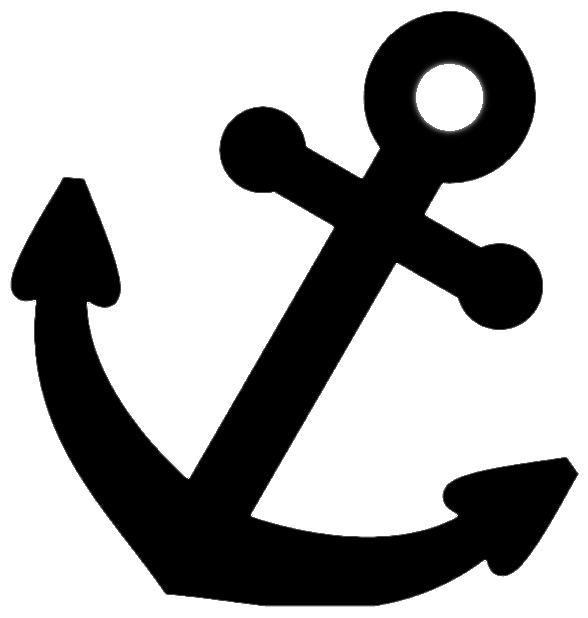
\includegraphics[width=1.5cm]{images/kotwica.png}}
}
\fancypagestyle{poezja}{%
    \pagestyle{plain}
    \fancyhead[R]{Poezja śpiewana}
    \fancyfoot[LO]{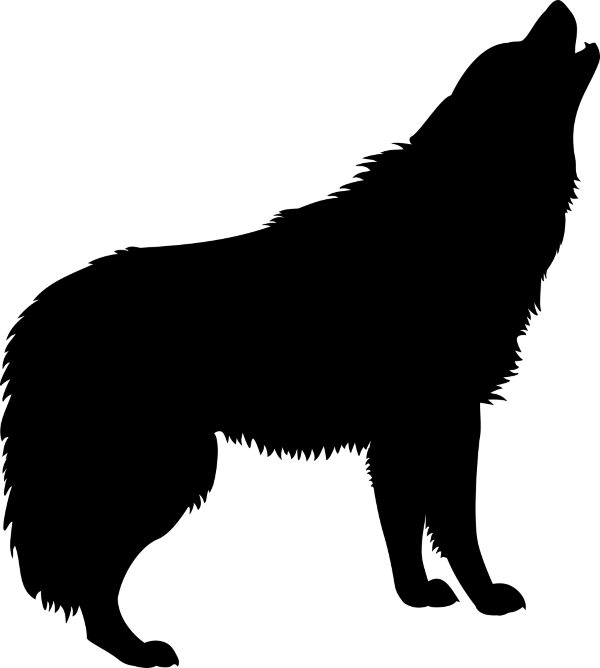
\includegraphics[width=1.5cm]{images/wilk.png}}
    \fancyfoot[RE]{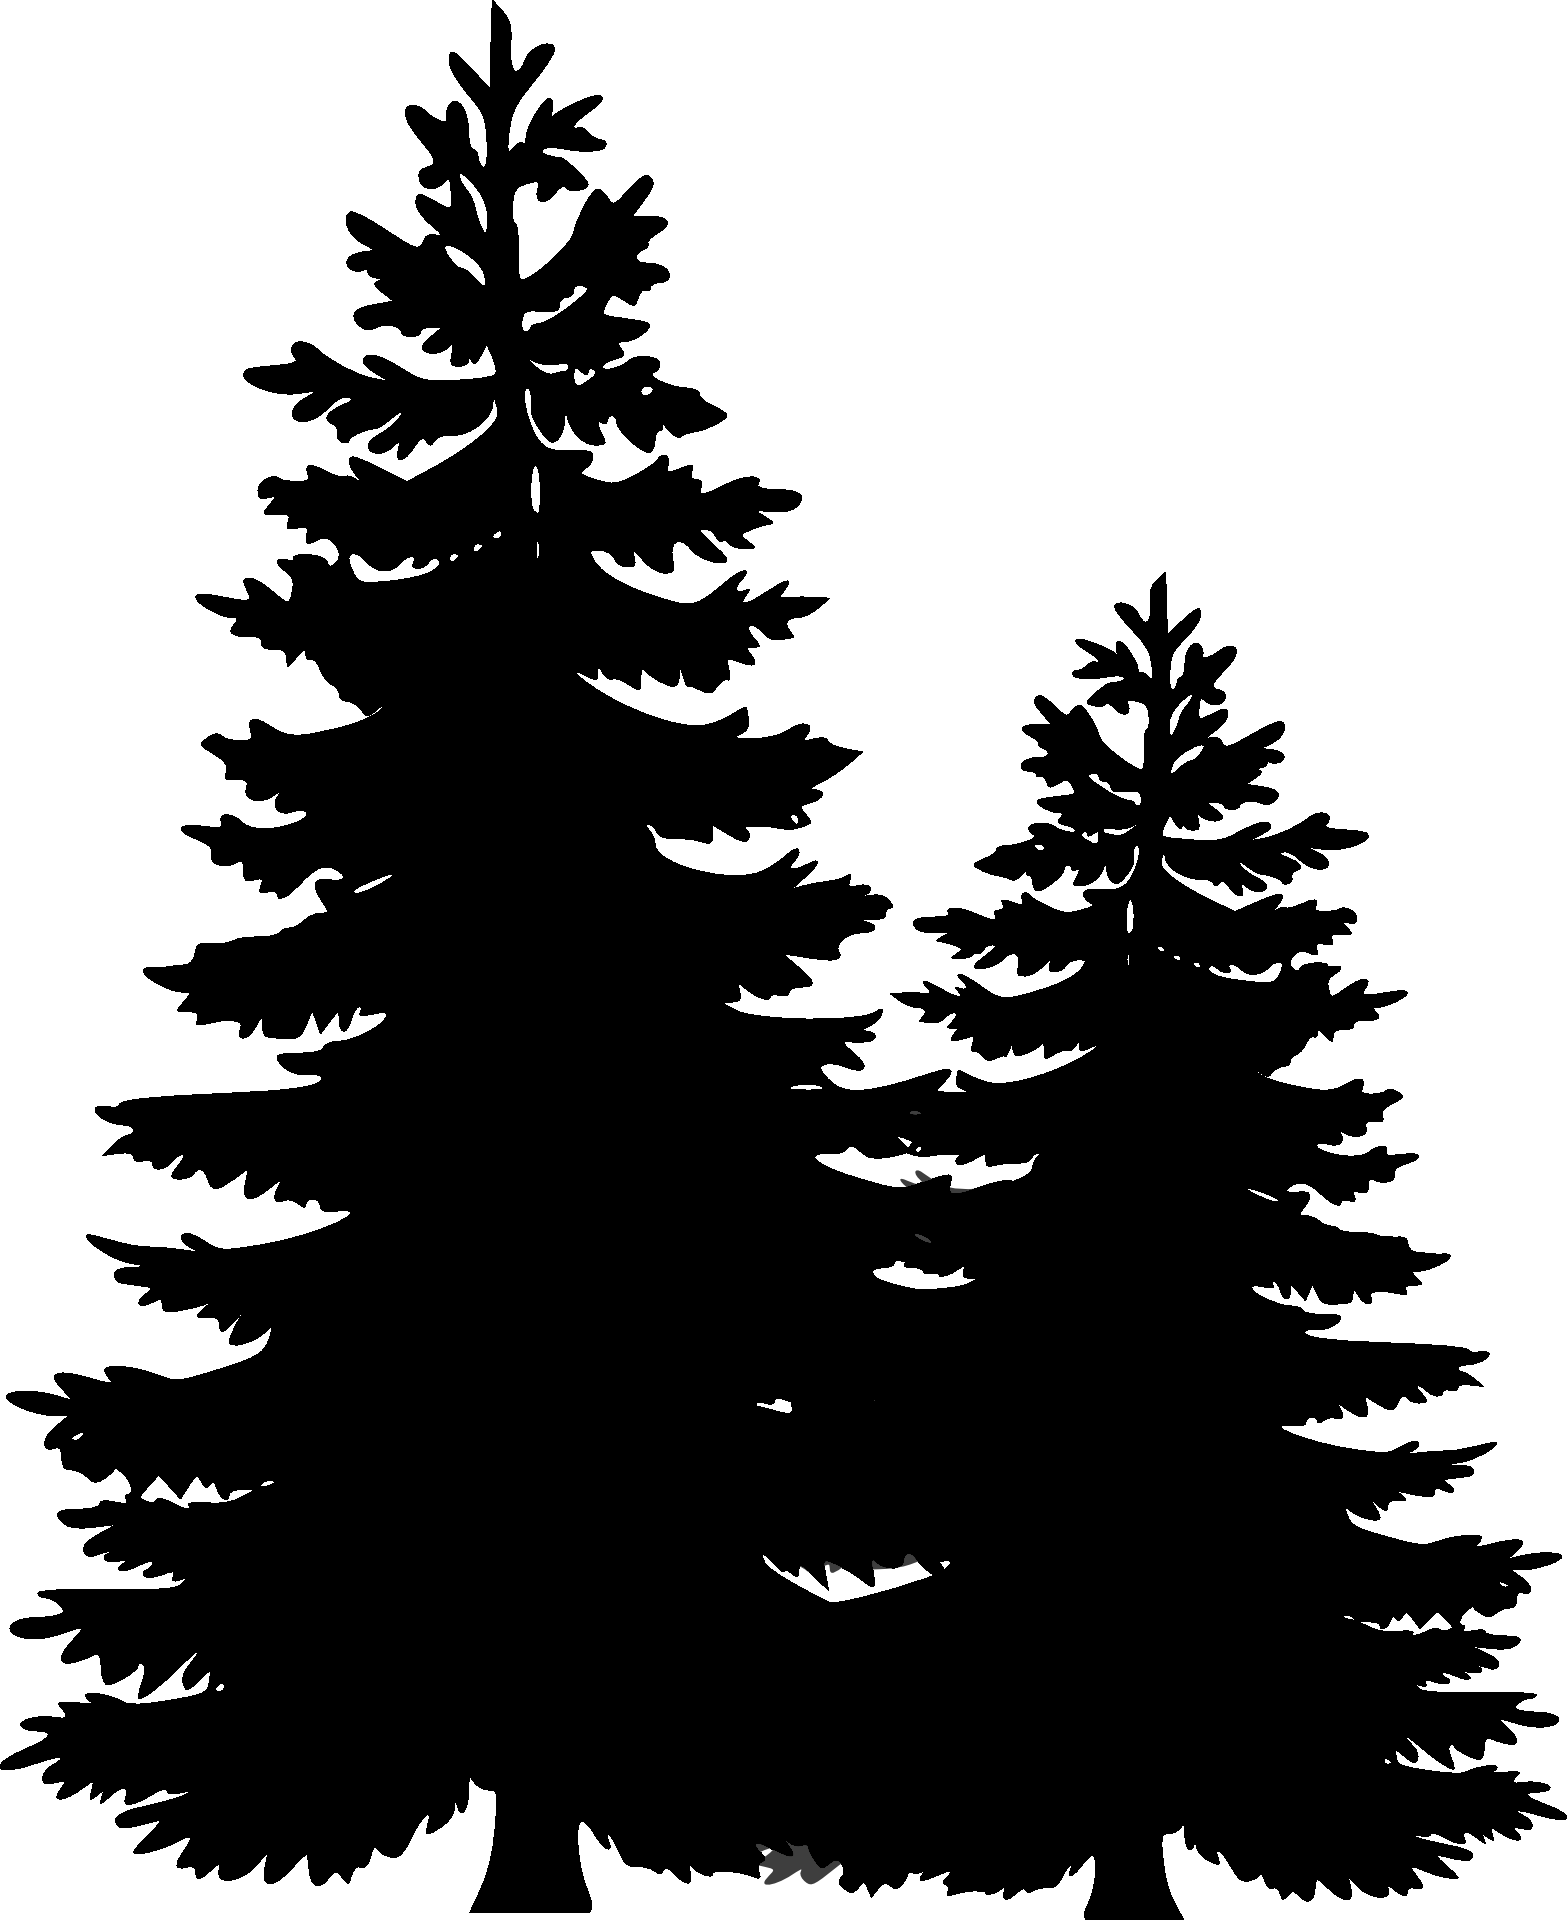
\includegraphics[width=1.5cm]{images/drzewa.png}}
}
\fancypagestyle{pop}{%
    \pagestyle{plain}
    \fancyhead[R]{Pop}
    \fancyfoot[LO]{
\includegraphics[width=1.5cm]{images/gwiazdy.png}}
    \fancyfoot[RE]{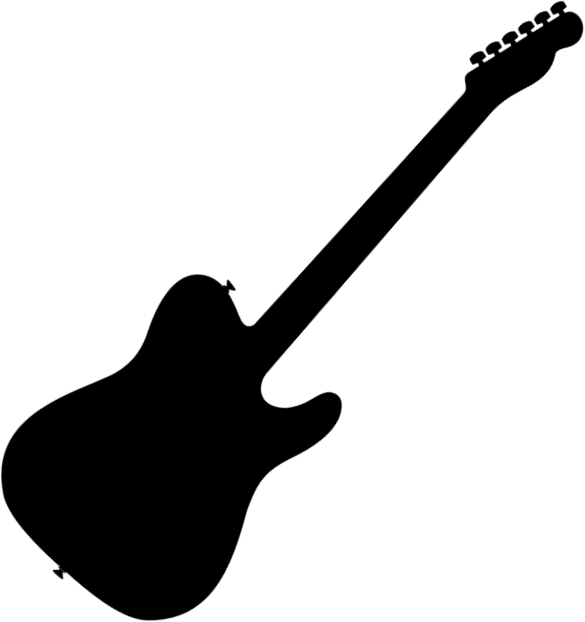
\includegraphics[width=1.5cm]{images/gitara.png}}
}

\renewcommand{\cftdot}{\ensuremath{\sim}}
\renewcommand{\cftsecleader}{\cftdotfill{\cftdotsep}}

% Usunięcie numeru rozdziału sprzed numeru sekcji
%\renewcommand{\thesection}{\arabic{section}}

\titleformat{\chapter}[block]{\centering\vspace{6cm}}{}{0pt}{\Huge\bfseries}

\begin{document}

\begin{titlepage}
    \begin{center}
        \vspace*{5cm}
        
        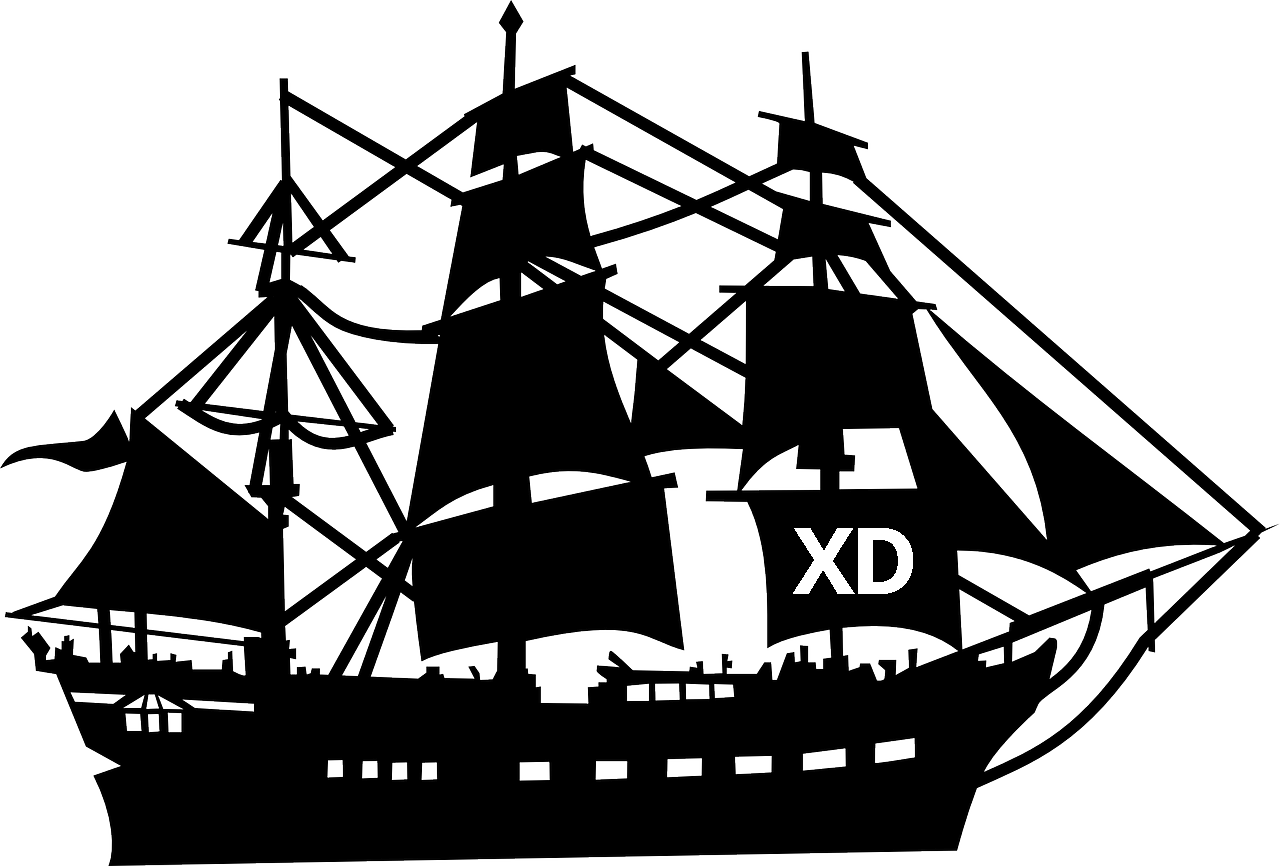
\includegraphics[height=8cm]{images/front-obrazek.png}

        \vspace{1.5cm}

        \Huge\textbf{Jakieś piosenki}
        
        \vspace{0.5cm}
        
        \LARGE Wydanie pierwsze
        
        \vfill

        \Large
        Wydawnictwo Kis Inkris \\
        Warszawa, 2021

        \vspace{0.5cm}

        \footnotesize
        https://github.com/dzierzanowski/spiewnik-szant

        \begin{tikzpicture}[remember picture,overlay,shift={(current page.south east)}]
            \node[anchor=south east,xshift=0cm,yshift=0cm]{
\includegraphics[width=3.5cm]{images/qr.png}};
        \end{tikzpicture}
    \end{center}
\end{titlepage}

\tableofcontents

\chapter{Szanty}
\begin{center}
    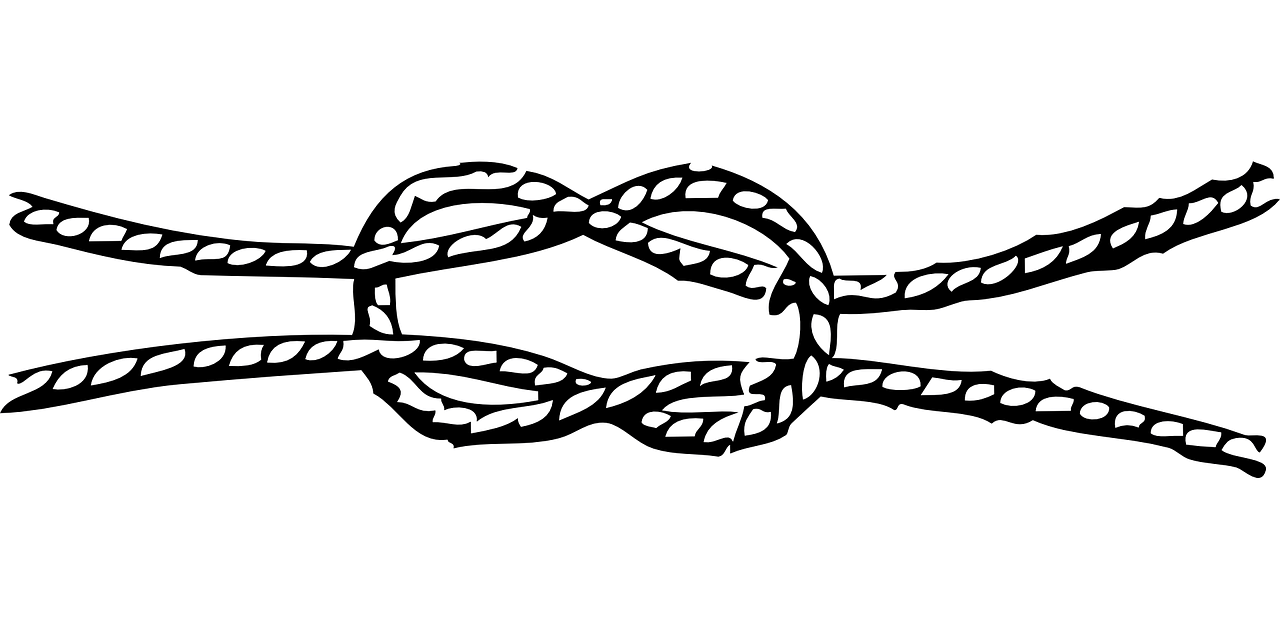
\includegraphics[width=0.5\textwidth]{images/wezel.png}
\end{center}
\pagestyle{szanty}
\newpage
\begin{song}{title={Chłopcy z Botany Bay}, music={Mietek Folk}, capo=3}
\begin{multicols}{2}
    \begin{verse}
        Już nad ^{h}Hornem ^{A}zapada ^{h}noc ^{h} \\
        Wiatr na ^{h}żaglach ^{A}położył ^{D}się ^{D} \\
        |: A tam ^{G}jeszcze ^{A}korsarze na ^*{D}Bota ^{A}ny ^{h}Bay | \\
        | Upy^{G}chają ^{A}zdobycze ^{h}swe :|
    \end{verse}
    \begin{verse}
        Jolly Roger na maszcie już śpi \\
        Jutro przyjdzie z Hiszpanem się bić \\
        A korsarze znużeni na Botany Bay \\
        Za zwycięstwo dziś będa swe pić
    \end{verse}
    \begin{verse}
        Śniady Clark puchar wznosi do ust \\
        "Bracia, toast! Niech idzie na dno!" \\
        Tylko Johnny nie pije, bo kilka mil stąd \\
        Otuliło złe morze go
    \end{verse}
    \begin{verse}
        Nie podnosi kielicha do ust \\
        Zawsze on tu najgłośniej się śmiał \\
        Mistrz fechtunku z Florencji ugodził go \\
        Już nie będzie za szoty się brał
    \end{verse}
    \begin{verse}
        W starym porcie zapłacze Margot \\
        Jej kochany nie wróci już \\
        Za dezercję do panny na kei w Brisbane \\
        Oddać musiał swą głowę pod nóż
    \end{verse}
    \begin{verse}
        Tak niewielu zostało dziś ich \\
        Resztę zabrał Neptun pod dach \\
        Choć na ustach wciąż uśmiech, to w sercach lód \\
        W kuflu miesza się rum i strach
    \end{verse}
    \begin{verse}
        To ostatni chyba już rejs \\
        Cios sztyletem lub kula w pierś \\
        Bóg na szkuner w niebiosach zabierze ich \\
        Wszystkich chłopców z Botany Bay
    \end{verse}
    \begin{verse}
        Już nad Hornem zapada noc \\
        Wiatr na żaglach położył się \\
        A tam jeszcze korsarze na Botany Bay \\
        Upychają zdobycze swe
    \end{verse}
\end{multicols}
\end{song}


\newpage
\begin{song}{title={Few days}, music={Ryczące Dwudziestki}, annex}
\begin{multicols}{2}
    \begin{verse}
        O Panie, czemu w ziemi tkwię \\
        Hej raz, hej raz! \\
        I macham szuflą cały dzień? \\
        Hej, na morze czas!
    \end{verse}
    \begin{chorus}
        Mogę kopać tu dalej \\
        Few days, few days \\
        Mogę kopać przez dni parę \\
        Ale wracać chcę $\times 2$
    \end{chorus}
    \begin{verse}
        Tam każdy takie bajdy plótł \\
        Nie raz, nie raz \\
        Przekroczysz Jukon, złota w bród \\
        Hej, na morze czas!
    \end{verse}
    \begin{chorus}
        Mogę kopać tu dalej\ldots $\times 2$ 
    \end{chorus}
    \vfill\null\columnbreak{}
    \begin{verse}
        Wykopię jeszcze parę dziur \\
        Hej raz, hej raz \\
        Wytoczę płonnej skały wór \\
        Hej, na morze czas!
    \end{verse}
    \begin{chorus}
        Mogę kopać tu dalej\ldots $\times 2$ 
    \end{chorus}
    \begin{verse}
        Za żonę tu łopatę mam \\
        Już dość, już dość \\
        A zysk, że jej uzywam sam \\
        Hej, na morze czas!
    \end{verse}
    \begin{chorus}
        Mogę kopać tu dalej\ldots $\times 2$
    \end{chorus}
    \begin{verse}
        O Panie nie jest to Twój raj \\
        O nie, o nie \\
        Nadzieję innym głupcom daj \\
        Ja na morze chcę!
    \end{verse}
    \begin{chorus}
        Chociaż już mi wystarczy \\
        Few days, few days \\
        Dam Ci jeszcze jedną szansę \\
        Ale wracać chcę $\times 2$
    \end{chorus}
\end{multicols}
\end{song}


\newpage
\begin{song}{title={Kapitan Kidd}, music={North Cape}}
\begin{multicols}{2}
    \begin{chorus}
        Me ^{e}imię ^{h}William ^{e}Kidd \\
        Już czeka ^{a}stryk, czeka ^{D}stryk \\
        Królewski ^{e}korsarz ^{h}William ^{e}Kidd, czeka ^*{G}stry ^{D}k \\
        Me ^{G}imię ^{D}William ^{a}Kidd \\
        Zbrodni ^*{e}ogrom ^{h}nych to ^{a}mit \\
        Powró^{e}ciłem, ^{G}choć w Lon^{h}dynie ^{D/F#}czeka ^{e}stryk
    \end{chorus}
    \begin{verse}
        Mój ^{e}ojciec ^{h}uczył ^{e}mnie \\
        Jak nie ^{G}znaleźć się na ^{D}dnie \\
        Lecz los o^{e}krutny ^{D}zabrał ^{a}go ro^{h}dzinie ^{e}mej \\
        Choć biblię w ^{e}rękę ^{h}moją ^{e}kładł \\
        Morza ^{G}urok na mnie ^{D}padł \\
        I mary^{e}narzem ^{D}stałem ^{a}się, choć ^{h}czeka ^{e}stryk
    \end{verse}
    \begin{chorus}
        Me imię William Kidd\ldots
    \end{chorus}
    \begin{verse}
        Kanonier William Moore \\
        Pierwszy trafił na mój sznur \\
        Bo przeciw mnie ośmielił się on wzniecić bunt \\
        Choć dobrym strzelcem William był \\
        Pod salingiem będzie gnił \\
        Buntownik każdy skończy tak, już czeka stryk
    \end{verse}
    \begin{chorus}
        Me imię William Kidd\ldots
    \end{chorus}
    \begin{verse}
        Raz gdy było ze mną źle \\
        Obiecałem sobie, że \\
        Mądrości drogą odtąd pójdę po kres dni \\
        Lecz mój korsarski podły fach \\
        Zabił wnet o duszę strach \\
        I potępienie czeka mnie, bo czeka stryk
    \end{verse}
    \begin{chorus}
        Me imię William Kidd\ldots
    \end{chorus}
    \begin{verse}
        \textit{(wolniej)} \\
        To egzekucyjny blok \\
        Zaraz mnie ogarnie mrok \\
        Bo na mą szyję kat założy gruby sznur \\
        Więc dzisiaj ostrzec ciebie chcę \\
        Byś za przykład nie brał mnie \\
        Mądrości drogą zawsze szedł, bo czeka stryk
    \end{verse}
    \begin{chorus}
        \textit{(szybciej)} \\
        Me imię William Kidd\ldots
    \end{chorus}
\end{multicols}
\end{song}
\newpage

\newpage
\begin{song}{title={Pij za starego (Whiskey in the jar)}, music={Thin Lizzy}, interpret={Poszedłem Na Dziób}}
    \begin{intro}
        \writechord{F} \writechord{C} \writechord{G} \writechord{C}
    \end{intro}
    \begin{multicols}{2}
    \begin{verse}
        Pły^{C}nąłem w dół Cork City \\
        By ^{a}przejść przez Góry Kerry \\
        Spot^{F}kałem tam Farrella \\
        Co ^{C}forsę swoją liczył \\
        Sięg^{C}nąłem więc po spluwę \\
        A ^{a}potem po swój rapier \\
        Krzyk^{F}nąłem: \say{Dawaj forsę \\
        Jeśli ^{C}ci miłe życie!}
    \end{verse}
    \begin{chorus}
        $\times 2$ \\
        Masza ^{G}ring dama du dama da \\
        ^{C} Pij za starego \\
        ^{F} Pij za starego \\
        Bo ^{C}whiskey ^{G}pełny ^{C}słój
    \end{chorus}
    \begin{interlude}
        \writechord{F} \writechord{C} \writechord{G} \writechord{C}
    \end{interlude}
    \vfill\null\columnbreak{}
    \begin{verse}
        Zabrałem całą forsę \\
        A trochę tego było \\
        Zaniosłem worek szmalu \\
        Do domu pięknej Molly \\
        A ona przysięgała \\
        Że tylko o mnie śniła \\
        Lecz wnet się okazało \\
        Że tylko szmal mój woli
    \end{verse}
    \begin{chorus}
        Masza ring dama du dama da\ldots
    \end{chorus}
    \begin{interlude}
        \writechord{F} \writechord{C} \writechord{G} \writechord{C}
    \end{interlude}
    \begin{verse}
        Pijany i zmęczony \\
        Poszedłem znów do Molly \\
        Zabrałem jej szmal cały \\
        Nie wiedząc, co mnie czeka \\
        Lecz nagle tuż przede mną \\
        Kapitan Farrell stoi \\
        Strzeliłem więc z mej spluwy \\
        Trafiając w tego człeka
    \end{verse}
    \begin{chorus}
        Masza ring dama du dama da\ldots
    \end{chorus}
    \begin{interlude}
        \writechord{F} \writechord{C} \writechord{G} \writechord{C}
    \end{interlude}
    \begin{verse}
        Rybacy łowią ryby \\
        Myśliwi tną zwierzynę \\
        A ja lubię posłuchać \\
        Odgłosu kanonady \\
        I lubię mieć przy sobie \\
        Mą Molly, cud-dziewczynę \\
        Lecz teraz siedzę w celi \\
        I mam łańcuchów ślady
    \end{verse}
    \begin{chorus}
        Masza ring dama du dama da\ldots
    \end{chorus}
    \begin{interlude}
        \writechord{F} \writechord{C} \writechord{G} \writechord{C}
    \end{interlude}
    \end{multicols}
\end{song}


\newpage
\begin{song}{title={Press gang (Branka)}, music={Cztery refy}}
\begin{multicols}{2}
    \begin{verse}
        W dół od rzeki, poprzez London Street \\
        Psów królewskich oddział zwarty szedł \\
        Ojczyźnie trzeba dziś świeżej krwi \\
        Marynarzy floty wojennej
    \end{verse}
    \begin{verse}
        A że byłem wtedy silny chłop\\
        W tłumie złowił mnie sierżanta wzrok \\
        W kajdanach z bramy wywlekli mnie \\
        Marynarza floty wojennej
    \end{verse}
    \begin{verse}
        Jak o prawa upominać się \\
        Na gretingu nauczyli mnie \\
        Niejeden krwią wtedy spłynął grzbiet \\
        Marynarza floty wojennej
    \end{verse}
    \begin{verse}
        Nikt nie zliczy ile krwi i łez \\
        Wsiąkło w pokład, gdy się zaczął rejs \\
        Dla chwały twej, słodki kraju mój \\
        Marynarzy floty wojennej
    \end{verse}
    \begin{verse}
        Hen, za rufą miły został dom \\
        Jesteś tylko parą silnych rąk \\
        Dowódca tu twoim bogiem jest \\
        Marynarzu floty wojennej
    \end{verse}
    \begin{verse}
        Gdy łapaczy szyk formuje się \\
        W pierwszym rzędzie możesz ujrzeć mnie \\
        Kto stanie na mojej drodze dziś \\
        \textbf{Łup} stanowi floty wojennej
    \end{verse}
\end{multicols}
    \includegraphics[width=\textwidth]{sheet\string_music/cztery\string_refy-press\string_gang.png}
\end{song}

\newpage
\begin{song}{title={Stary bryg}, music={EKT Gdynia}}
    \begin{intro}
        \writechord{d} \writechord{a} \writechord{d} \writechord{G} $\times 2$
    \end{intro}
    \begin{verse}
        ^{d} Gdy wy^{a}pływał z ^{d}portu ^{a}stary bryg ^{d} ^{a} ^{d} ^{G} \\
        ^{d}Jego ^{C}dalszych ^{F}losów ^{C}nie znał ^{d}nikt ^{a} ^{d} ^{G} \\
        ^{d}Nikt nie wiedział ^{F}o tym, że \\
        ^{G}Statkiem-widmem ^{a}stanie się stary ^{d}bryg ^{a} ^{d} ^{G} \\
        ^{d} ^{a} ^{d} ^{G}
    \end{verse}
    \begin{chorus}
        ^{d}Hej, ^{F}ho! ^{C}na umrzyka ^{d}skrzyni \\
        ^{F}I bu^{C}telka ^{d}rumu ^{a} ^{d} ^{G} \\
        ^{d}Hej, ^{F}ho! ^{C}resztę czas u^{d}czyni \\
        ^{F}I bu^{C}telka ^{d}rumu ^{a} ^{d} ^{G} \\
        ^{d} ^{a} ^{d} ^{G}
    \end{chorus}
    \begin{verse}
        Co z załogą zrobił stary bryg \\
        Tego też nie zgadnie chyba nikt \\
        Czy zostawił w porcie ją \\
        Czy na morza dnie? Nikt nie wie gdzie
    \end{verse}
    \begin{chorus}
        Hej, ho! na umrzyka skrzyni\ldots
    \end{chorus}
    \begin{verse}
        Przepowiednia zła jest, że ho ho \\
        Kto go spotka, marny jego los \\
        Ale my nie martwmy się \\
        Hej, nie martwmy się --- rum jeszcze jest!
    \end{verse}
    \begin{chorus}
        Hej, ho! na umrzyka skrzyni\ldots $\times 2$ 
    \end{chorus}
\end{song}


\newpage
\begin{song}{title={Stary wrak}, music={Mechanicy Szanty}}
\small
    \begin{intro}
        \writechord{d} \writechord{a} \\
        \writechord{C} \writechord{D}\writechord{G} \\
        \writechord{a} \writechord{G} \writechord{asus2}
    \end{intro}
    \begin{multicols}{2}
    \begin{verse}
        Już za^{d}kończył życie swe ^{a} \\
        Oparł ^{C}dziób o stro^{D}my ^{G}brzeg \\
        Rejsu ^{a}kres wyznaczył cz^{G}as i morza gniew ^{asus2} \\
        Już pozostał tylko ślad \\
        Żagli, które targał wiatr \\
        Nie zawiodą go już więcej na swój szlak \\
        \\
        Tam gdzieś ^{a}czeka na nas znów \\
        Żagli ^{G}biel i silny wiatr \\
        Tam gdzieś ^{a}czeka żywioł, który wciąż nas ^{F}gna \\
        Gdzieś do ^{d}postrzępionych pa^{a}lm \\
        Do mil^{C}czących, zło^{D}tych ^{G}plaż \\
        Stary ^{a}wrak na pokład j^{G}uż nie weźmie nas ^{asus2}
    \end{verse}
    \begin{center}
        \vspace{0.6cm}
        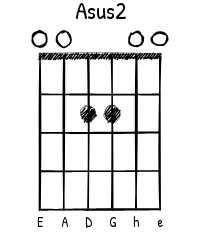
\includegraphics[height=3.5cm]{images/Asus2.png}
    \end{center}
    \vfill\null\columnbreak{}
    \begin{verse}
        Dzielny był przez tyle lat \\
        ``Czarnej Kuli'' nosił znak \\
        Imię jego wśród liniowców każdy znał \\
        Gdy na cumach w porcie stał \\
        Smukłe linie, piękny kształt \\
        Każdy morze razem z nim zdobywać chciał \\
        \\
        Płynąć tam, gdzie czeka znów \\
        Żagli biel i silny wiatr \\
        Płynąć tam, gdzie żywioł, który wciąż nas gna \\
        Gdzieś do postrzępionych palm \\
        Do milczących, złotych plaż \\
        Dziś na pokład stary wrak nie weźmie nas
    \end{verse}
    \begin{verse}
        To wędrówki jego kres \\
        Skończył się już żagli wiek \\
        Nie powrócą pod błękitny nieba dach \\
        Tylko w sercach naszych trwa \\
        Do żaglowców z tamtych lat \\
        Wielka miłość, która w morze ciągnie nas \\
        \\
        Chcemy płynąć tam, gdzie znów \\
        Żagli biel i silny wiatr \\
        Chcemy płynąć w żywioł, który wciąż nas gna \\
        Tam do postrzępionych palm \\
        Do milczących, złotych plaż \\
        Stary wrak wciąż pływać będzie w naszych snach
    \end{verse}
    \begin{interlude}
        Tam do postrzępionych palm \\
        Do milczących, złotych plaż \\
        Stary wrak wciąż pływać będzie w naszych snach
    \end{interlude}
    \end{multicols}
\end{song}



\chapter{Poezja śpiewana}
\begin{center}
    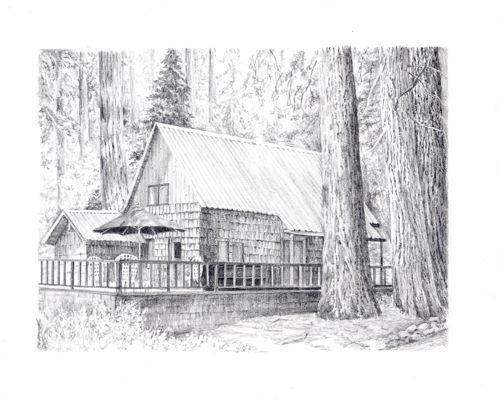
\includegraphics[width=0.5\textwidth]{images/chatka.jpg}
\end{center}
\pagestyle{poezja}
\newpage
\begin{song}{title={Pójdę w połoniny (A ja wolę…)}, music={Dom o Zielonych Progach}}
    \begin{verse}
        ^{E} A ja ^{a}wolę \\
        ^{E} Na zielonej ^{a}łące ^*{G}sie ^{F}dzieć \\
        Niźli w ^{C}szarym mieście, które ^{E} głuche jest \\
        ^{F} Na moje wo^{C}łanie \\
        ^{F} Na mój niemy ^{C}krzyk \\
        ^{F} Na moją sa^{C}motność obo^{E}jętne ^{a}jest ^{G} ^{F} ^{C}
    \end{verse}
    \begin{verse}
        Pójdę w połoniny \\
        W roztańczone bujne trawy \\
        Pod rękę razem z polnym wiatrem \\
        Między szumem liści \\
        Ukryte słowa dla mnie \\
        Zanucę je głośniej, niech popłyną dalej gdzieś
    \end{verse}
    \begin{verse}
        Niech na moim niebie \\
        Rozniebieszczą się gwiazdy \\
        Niczym Mały Książę będę sobie szedł \\
        Może spotkam różę \\
        Której kolców brak \\
        Która zdradzi mi swe imię i swój uśmiech da
    \end{verse}
    \begin{interlude}
        Na na na na na\ldots
    \end{interlude}
    \begin{verse}
        Pójdę w połoniny\ldots
    \end{verse}
\end{song}


\newpage
\begin{song}{title={Wilcza zamieć}, music={Marcin Przybyłowicz (z gry Wiedźmin: Dziki Gon)}, interpret={Studio Accantus}}
    \begin{intro}
        \writechord{d} \writechord{d} \writechord{B} \writechord{C} $\times 2$
    \end{intro}
    \begin{verse}
        Na ^{d}szlak moich blizn po^{B}prowadź ^{C}palec \\
        By ^{d}nasze drogi spleść ^{g}gwiazdom na ^{A}przekór \\
        ^{B} Otwórz te rany, ^{g} a potem ^{A}zalecz \\
        ^{d}Aż w zawiły losu ułożą się wzór
    \end{verse}
    \begin{chorus}
        Z moich ^{d}snów uciekasz nad ranem \\
        Cierpka ^{B}jak agrest, słodka jak bez ^{C} \\
        Chcę ^{d}śnić czarne loki splątane \\
        ^{B}Fiołkowe oczy ^{g}mokre od ^{A}łez
        \\
    \end{chorus}
    \begin{verse}
        Za wilczym śladem podążę w zamieć \\
        I twoje serce wytropię uparte \\
        Przez gniew i smutek stwardniałe w kamień \\
        Rozpalę usta smagane wiatrem
    \end{verse}
    \begin{chorus}
        Z moich snów uciekasz nad ranem\ldots
    \end{chorus}
    \begin{verse}
        Nie wiem czy jesteś moim przeznaczeniem \\
        Czy przez ślepy traf miłość nas związała \\
        Kiedy wyrzekłem moje życzenie \\
        Czyś mnie wbrew sobie wtedy pokochała?
    \end{verse}
    \begin{chorus}
        Z moich snów uciekasz nad ranem\ldots
    \end{chorus}
    \begin{interlude}
        \writechord{d} \writechord{d} \writechord{B} \writechord{C} $\times 2$
    \end{interlude}
\end{song}


\newpage
\begin{song}{title={1788}, music={Jacek Kaczmarski}}
    \small
    \begin{intro}
        \writechord{F} \writechord{B} \writechord{F} \writechord{C} \\ 
        \writechord{F} \writechord{B} \writechord{F} \writechord{C} \writechord{F}
    \end{intro}
    \begin{multicols}{2}
\begin{verse}
^{F}Ta pierwsza morska ^{B}podróż do Australii! \\
^{F}Łotry przy burtach, prosty^{C}tutki w kojach \\
^{F}Wszyscy się bali, łk^{B}ali i rzygali \\
^{F}W drodze do raju. Przewrot^{C}ności Twoja \\
^{d}Panie, coś w jeszcze nam niezn^{g}anych planach \\
^{d} Miał czarne diabły strzeg^{a}ące wybrzeży \\
^{B}Edenu, który prz^{C}eznaczyłeś ^{F}dla nas \\
A w kt^{B}óry nikt, prawdę ^{C}mówiąc, nie ^{d}wierzył! \\
\\
^{d} ^{B} ^{F} ^{C}
\end{verse}
\begin{verse}
Czym żeśmy, marni, zasłużyli na to? \\
Ten, co zawisnąć miał za kradzież płaszcza \\
Płakał nad swoją niechybną zatratą \\
Nie widział Ciebie w robaczywych masztach \\
Statku, co tylko był więzieniem nowym \\
Tej co kupczyła ciałami swych dziatek \\ 
Ani przez mgnienie nie przyszło do głowy \\
Że to nadziei - nie rozpaczy statek \\
\end{verse}
\begin{verse}
Niejeden żołnierz z ponurej eskorty \\
Bo czym się ich los od naszego różnił? \\ 
Wiedział, że nigdy już nie ujrzy portu \\
Gdzie go podejmą karczmarze usłużni \\ 
I płatne dziewki; że zabraknie rumu \\
Zanim do celu przygnasz okręt szparki \\
Z marynarzami pili więc na umór \\
I - wbrew zakazom - grali o więźniarki \\
\end{verse}
\begin{verse}
Prawda, nie wszyscy próby Twe przetrwali \\
Ale też ciężkoś nas doświadczał, Panie \\
Nie oszczędzałeś nam wysokiej fali \\ 
Za którą mnogim przyszło w oceanie \\
Zakończyć żywot; innym dziąsła zgniły \\
Wypadły zęby, rozgorzały wrzody \\ 
Więc znaczą nasz zielony szlak mogiły \\
Szkorbutu, szału, francuskiej choroby \\
\end{verse}
\begin{verse}
Nikt nie odnajdzie w ruchomych otchłaniach \\
Ciał nieszczęśników - oprócz Ciebie, Boże \\
Ich żywot grzeszny epitafiów wzbrania \\
Lecz - ukarani. Więc wystarczy może \\ 
Żeś się posłużył straszliwym przykładem \\
Oni naprawdę dotarli do piekieł \\
A umierając nie wierzył z nich żaden \\
Że w swym cierpieniu umiera - człowiekiem \\
\end{verse}
\begin{verse}
Ląd nam się wydał niegościnny, dziki \\
Łotr bez honoru, kobieta sprzedajna \\
Z dnia na dzień - jak się stać ma osadnikiem \\
Nieznanych światów? Bo rozpoznać Raj nam \\
Nie było łatwo; znaleźć w sobie siłę \\
Wbrew przeciwnościom, bez słowa zachęty \\
By mimo wszystko żyć - nim nam odkryłeś \\ 
Kraj szczodry w zboże, złoto i diamenty \\
\end{verse}
\begin{verse}
^{d}Łajdacki pomiot, łot^{g}rowskie nasienie \\
^{d}Czerpiąc ze spichrza Twoich d^{a}óbr wszelakich \\
^{B}Choć tyle wiemy w^{C}łasnym doświadcz^{F}eniem \\
^{d}W nas jest Raj, Pi^{B}ekło - ^{F}I do obu-szl^{C}aki \\
^{d}W nas jest Raj, Pi^{B}ekło - ^{F}I do obu-szl^{C}aki \\
^{d}W nas jest Raj, Pi^{B}ekło - ^{F}I do obu-szl^{C}aki \\
\\
\writechord{d} \writechord{B} \writechord{F} \writechord{C}
\end{verse}
\end{multicols}
\begin{center}
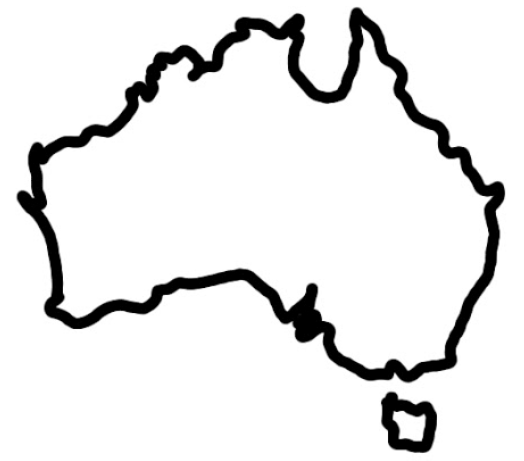
\includegraphics[width=0.15\textwidth]{images/1788.png}  
\end{center}
\end{song}
\newpage
\newpage\pagestyle{poezja}

\chapter{Pop}
\begin{center}
    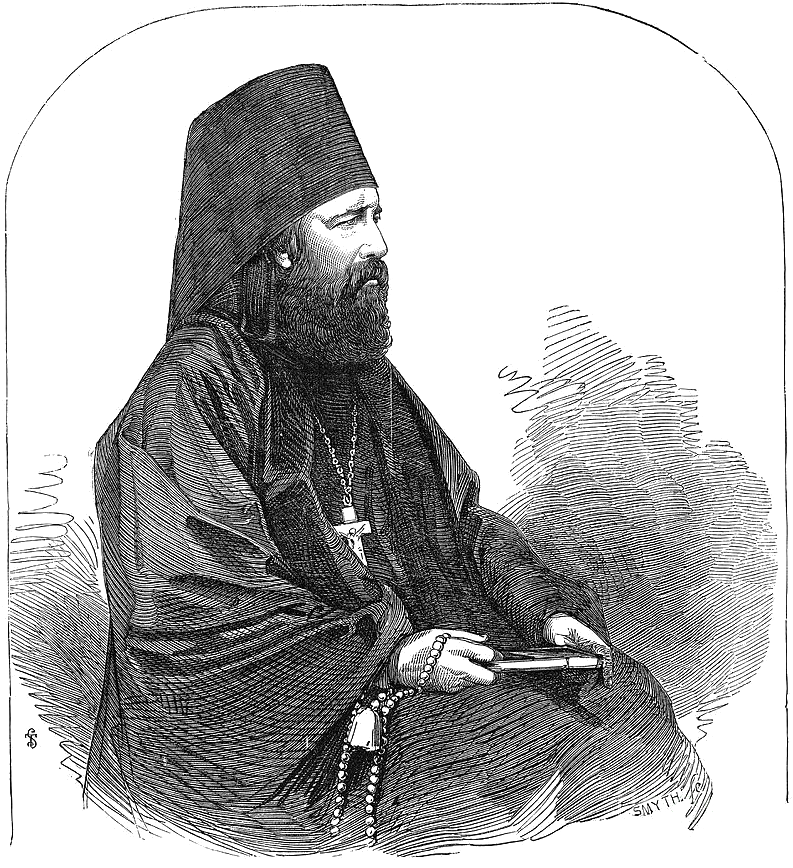
\includegraphics[width=0.4\textwidth]{images/pop.png}
\end{center}
\pagestyle{pop}
\newpage
\begin{song}{title={Byłaś serca biciem}, music={Jerzy Dobrzyński}, interpret={Andrzej Zaucha}, capo=3}
    \begin{intro}
    \writechord{a} \writechord{G} \writechord{d7} \writechord{d7}
    \end{intro}
    \begin{chorus}
        ^{a}Byłaś serca b^{G}iciem ^{d7} \\
        ^{a}Wiosną, zimą, ż^{G}yciem ^{d7} \\
        ^{a}Marzeń moich e^{G}chem ^{d7} \\
        ^{a}Winem, wiatrem, śmi^{G}echem ^{d7}
    \end{chorus}
    \begin{verse}
        Ostatnio w ^{a}mieście mym tramwaje ^{G}po północy b^{d7}łądzą \\
        Rozkładem n^{a}ocnych tras piekielne ^{G}jakieś moce rz^{d7}ądzą \\
        Nie wiedzieć ^{a}czemu wciąż rozkł^{G}ady jazdy ta^{d7}k zmieniają \\
        Że prawie k^{a}ażdy tramwaj ^{G}pod twym oknem ^{d7}nocą staje
    \end{verse}
      \begin{chorus}
        Byłaś serca biciem\ldots
    \end{chorus}
    \begin{verse}
        Ostatnio słońca mniej, ostatnio noce bardziej ciemne \\
        Już nawet księżyc drań o tobie nie chce gadać ze mną \\
        W kieszeni grosze dwa, w kieszeni na dwa szczęścia grosze \\
        W tym jednak losu żart, że ja obydwa grosze noszę
    \end{verse}
    \begin{chorus}
        Byłaś serca biciem\ldots
    \end{chorus}
    \begin{interlude}
        ^{F}Ktoś p^{d7}ytał jak się m^{C}asz, j^{a}ak się czujesz \\
        ^{F}Ktoś, z k^{d7}im rok w wojnę g^{C}rasz wycze^*{e}ku ^{A}je \\
        ^{F}Ktoś, k^{d7}to nocami, u^{C}licami, t^{a}ramwajami \\
        ^{F}Pod twe okno ^{d7}mknie, gdzie spo^*{D}ty ^{Eb}ka ^{E}mnie
    \end{interlude}
    \begin{chorus}
        Byłaś serca biciem\ldots
    \end{chorus}
    \begin{interlude}
        Ktoś pytał jak się masz\ldots
    \end{interlude}
\end{song}


\newpage
\small
\begin{song}{title={In the End}, music={Linkin Park}, capo={1}}
    \begin{intro}
        \writechord{d} \writechord{C} \writechord{B} \writechord{C} $\times 2$
    \end{intro}
    \begin{multicols}{2}
    \begin{verse}
        \textit{(It starts with\ldots)} \\
        ^{d}One thing, I don't know why \\
        It ^{C}doesn't even matter how hard you try \\
        Ke^{B}ep that in mind, I designed this rhyme \\
        To expla^{C}in in due time \textit{(all I know)} \\
        Time is a valuable thing \\
        Watch it fly by as the pendulum swings \\
        Watch it count down to the end of the day \\
        The clock ticks life away \textit{(it's so unreal)} \\
        Didn't look out below \\
        Watch the time go right out the window \\
        Tryin' to hold on, I didn't even know \\
        I wasted it all, just to\ldots \textit{(watch you go)} \\
        I kept everything inside \\
        And even though I tried, it all fell apart \\
        What it meant to me will eventually be \\
        A memory of a time, when\ldots
    \end{verse}
    \begin{chorus}
        I tried so ^{d}hard and got so f^{F}ar \\
        But in the e^{C}nd, it doesn't even ma^{B}tter \\
        I had to ^{d}fall to lose it a^{F}ll \\
        But in the e^{C}nd, it doesn't even ma^{B}tter
    \end{chorus}
    \vfill\null\columnbreak{}
    \begin{verse}
        One thing, I don't know why \\
        It doesn't even matter how hard you try \\
        Keep that in mind, I designed this rhyme \\
        To remind myself how\ldots \textit{(I tried so hard)} \\
        In spite of the way you were mockin' me \\
        Actin' like I was part of your property \\
        Rememberin' all the times you fought with me \\
        I'm surprised it\ldots \textit{(got so far)} \\
        Things aren't the way they were before \\
        You wouldn't even recognize me anymore \\
        Not that you knew me back then \\
        But it all comes back to me \textit{(in the end)} \\
        You kept everything inside \\
        And even though I tried, it all fell apart \\
        What it meant to me will eventually be \\
        A memory of a time when\ldots
    \end{verse}
    \begin{chorus}
        I tried so hard and got so far\ldots
    \end{chorus}
    \begin{interlude}
        I've put my tr^{d}ust in yo^{C}u \\
        Pushed as f^{B}ar as I can g^{C}o \\
        For all th^{d}is, there's only o^{C}ne thing you should ^*{B}kn ^{C}ow
    \end{interlude}
    \begin{info}
        \textit{(mocniej, głośniej, \textbf{drzeć ryja})} \\
        I've put my tr^{d}ust in yo^{F}u \\
        Pushed as f^{C}ar as I can g^{B}o \\
        For all th^{d}is, there's only o^{F}ne thing you should ^*{C}kn ^{B}ow
    \end{info}
    \begin{chorus}
        I tried so hard and got so far\ldots
    \end{chorus}
    \begin{interlude}
        \writechord{d} \writechord{C} \writechord{B} \writechord{C} $\times 2$
    \end{interlude}
    \end{multicols}
\end{song}


\newpage
\small
\begin{song}{title={Pomaluj moje sny}, music={Breakout}}
    \begin{info}
        (16-bar blues, A moll)
    \end{info}
    \begin{intro}
        \writechord{C} \writechord{C} \writechord{D} \writechord{D} \\
        \writechord{a5} \writechord{G} \writechord{a5} \writechord{G} $\times 2$
    \end{intro}
    \begin{multicols}{2}
    \begin{verse}
        ^{a5} Nie zazdroszczę łodzi żagla, kiedy wiatr ^{G} \\
        ^{a5} Gna po morzach ją dalekich, gna przez świat ^{G} \\
        ^{a5} Nie zazdroszczę ptakom skrzydeł, rybom płetw^{G} \\
        ^{a5} Bo najbardziej ponad wszystko pragnę mieć \\
        Pragnę ^{D5}mieć, ^{C} ^{D5} ^{C}pragnę ^{a5}mieć ^{G} ^{a5} ^{G}
    \end{verse}
    \begin{chorus}
        ^{C} Sny kolorowe, ^{D} pomaluj moje sny ^{a5} ^{G} ^{a5} ^{G}
    \end{chorus}
    \bigskip
    \begin{verse}
        Chcę zamieszkać w kolorowym mieście snu \\
        W kolorowym rwać ogrodzie bukiet bzów \\
        Dla dziewczyny kolorowej, która w pieśń \\
        Wszystkie barwy i odcienie umie wpleść \\
        Ja chcę śnić, ja chcę śnić
    \end{verse}
    \begin{chorus}
        Sny kolorowe, pomaluj moje sny
    \end{chorus}
    \begin{solo}
        (zwrotka + refren)
    \end{solo}
    \begin{verse}
        Tak, jak gdybym tego mało miał za dnia \\
        Tyle czerni w moich snach jest, tyle zła \\
        Daj mi proszę chociaż w nocy barwny sen \\
        Niech mi we śnie będzie jaśniej, niż jest w dzień \\
        Daj mi dziś, daj mi dziś
    \end{verse}
    \begin{chorus}
        Sny kolorowe, pomaluj moje sny $\times 4$
    \end{chorus}
    \vfill\null\columnbreak{}
    \begin{center}
      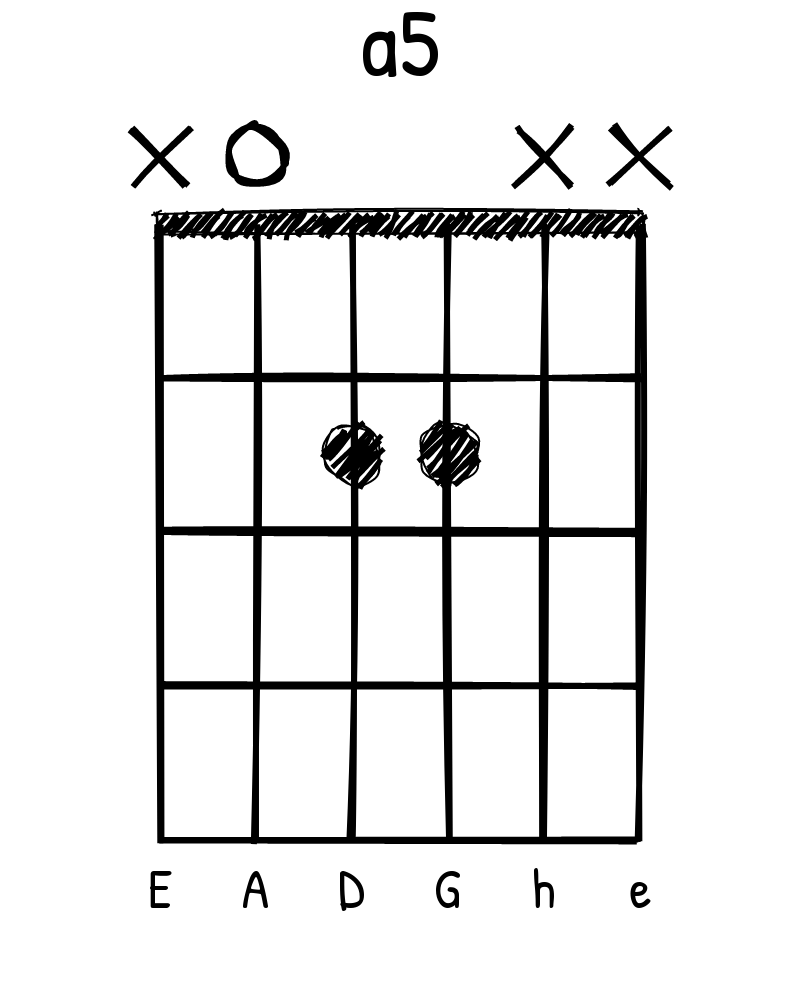
\includegraphics[height=3.5cm]{images/a5.png} \\
      \vspace{0.6cm}
      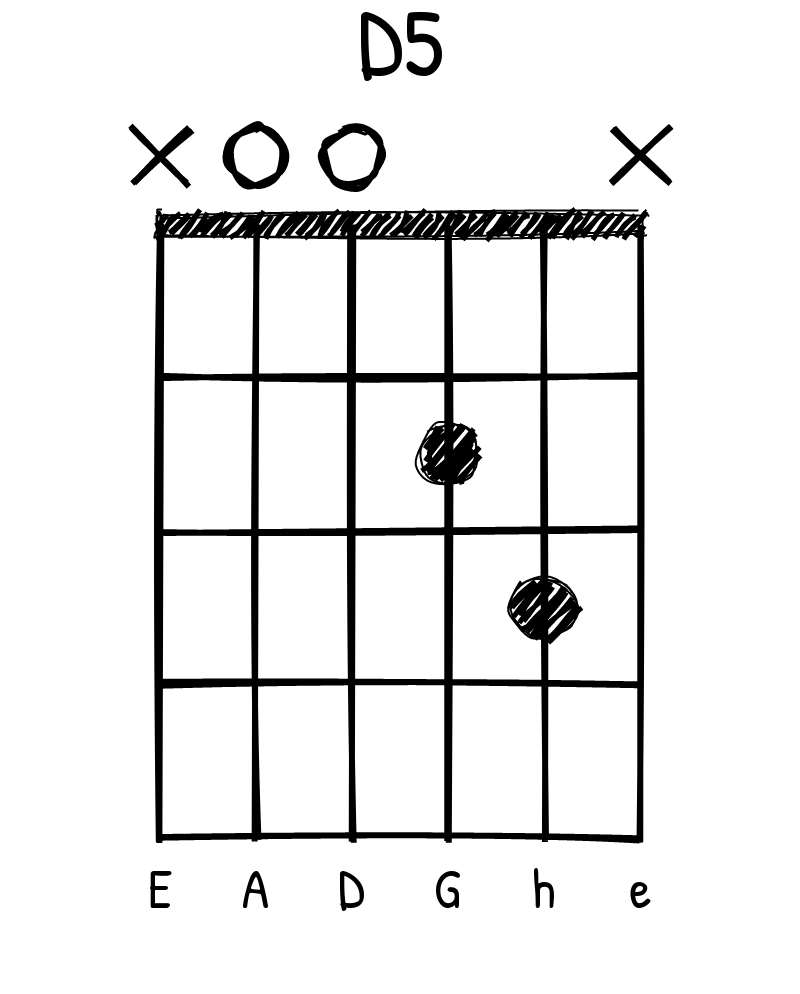
\includegraphics[height=3.5cm]{images/D5.png}
    \end{center}
    \end{multicols}
\end{song}


\newpage
\begin{song}{title={Premium Boy (Somebody That I Used To Know)}, music={Gotye}, interpret={808 Squad}}
\begin{multicols}{2}
    \small
    \begin{intro}
        \writechord{d} \writechord{C} \writechord{d} \writechord{C} $\times 4$
    \end{intro}
    \begin{verse}
        ^{d}Now and ^{C}then I think of ^{d}when we ^{C}were toge^{d}ther ^{C} ^{d} ^{C} \\
        ^{d} Like when you ^{C}said you felt so ^{d}happy ^{C}you could di^{d}e ^{C} ^{d} ^{C} \\
        ^{d} Told my^{C}self that you were ^{d}right for ^{C}me \\
        ^{d} But felt so ^{C}lonely in your ^{d}company ^{C} \\
        ^{d} But that was ^{C}love and it's an ^{d}ache I ^{C}still remem^{d}ber ^{C} ^{d} ^{C}
    \end{verse}
    \begin{interlude}
        \writechord{d} \writechord{C} \writechord{d} \writechord{C} $\times 4$
    \end{interlude}
    \begin{verse}
        You can get addicted to a certain kind of sadness \\
        Like resignation to the end, always the end \\
        So when we found that we could not make sense \\
        Well you said that we would still be friends \\
        But I'll admit that I was glad it was over
    \end{verse}
    \begin{chorus}
        ^{d} Bo ^{C}Michał to jest ^{B}premium ^{C}boy \\
        ^{d} Pije ^{C}kawę z mlekiem ^{B}sojowym gar^{C}dzi normal^{d}ną \\
        ^{C}Gardzi także ^*{B}herba ^{C}tą \\
        ^{d}Chyba że po^{C}słodzi cukrem ^*{B}trzcino ^{C}wym \\
        ^{d} Michał ^{C}to jest taki ^{B}premium ^{C}boy \\
        ^{d} Na jego ^{C}chlebie możesz ^{B}znaleźć tylko ^{C}  majo^{d}nez \\
        ^{C}Kiedyś zgłupiał ^{B}włączył ^{C}jazz \\
        ^{d}Potem wszedł na ^{C}łóżko i ze^{B}rzygał ^{C}się \\
        |: (bo Mi^{d}chał ^{C}--- to ^{B}premium bo^{C}y) | \\
        | ^{d}Każdy wie, że ^{C}Michał to jest ^{B}premium ^{C}boy :| \\
    \end{chorus}
    \begin{interlude}
        \writechord{d} \writechord{C} \writechord{d} \writechord{C} $\times 4$
    \end{interlude}
\end{multicols}
\end{song}



% Ostatnia strona parzysta pusta, żeby nie było tekstu na odwrocie
\clearpage{\mbox{}\pagestyle{empty}\cleardoublepage}

\end{document}
